\section{Simplification}

Two simplification functions are devised to reduce an input point set, either randomly or using a grid-based clustering approach.

Function \ccc{CGAL::random_simplify_point_set()} randomly deletes a user-specified fraction of points from the input point set. This algorithm is fast. \\
\ccRefIdfierPage{CGAL::random_simplify_point_set}  \\

The following example reads an input point set and randomly deletes 75\% of the points.
\ccIncludeExampleCode{Point_set_processing_3/random_simplification_example.cpp}

% PA: careful, if you first construct a grid and cluster all points lying in the same cell of the grid (by merging or whatever) it should be called grid_simplify
Function \ccc{CGAL::grid_simplify_point_set()} considers a regular grid covering the bounding box of the input point set, and clusters all points sharing the same cell of the grid by picking as representant one of the point arbitrarily chosen. This algorithm is slower than \ccc{CGAL::random_simplify_point_set()}. \\
% PA: can't you do better? ie pick the point which minimizes sum of squared distances to others?
% add example?
\ccRefIdfierPage{CGAL::grid_simplify_point_set}  \\

% Insert image merge_simplification.jpg/eps
\begin{center}
    \label{Point_set_processing_3-fig-merge_simplification}
    % Image
    \begin{ccTexOnly}
        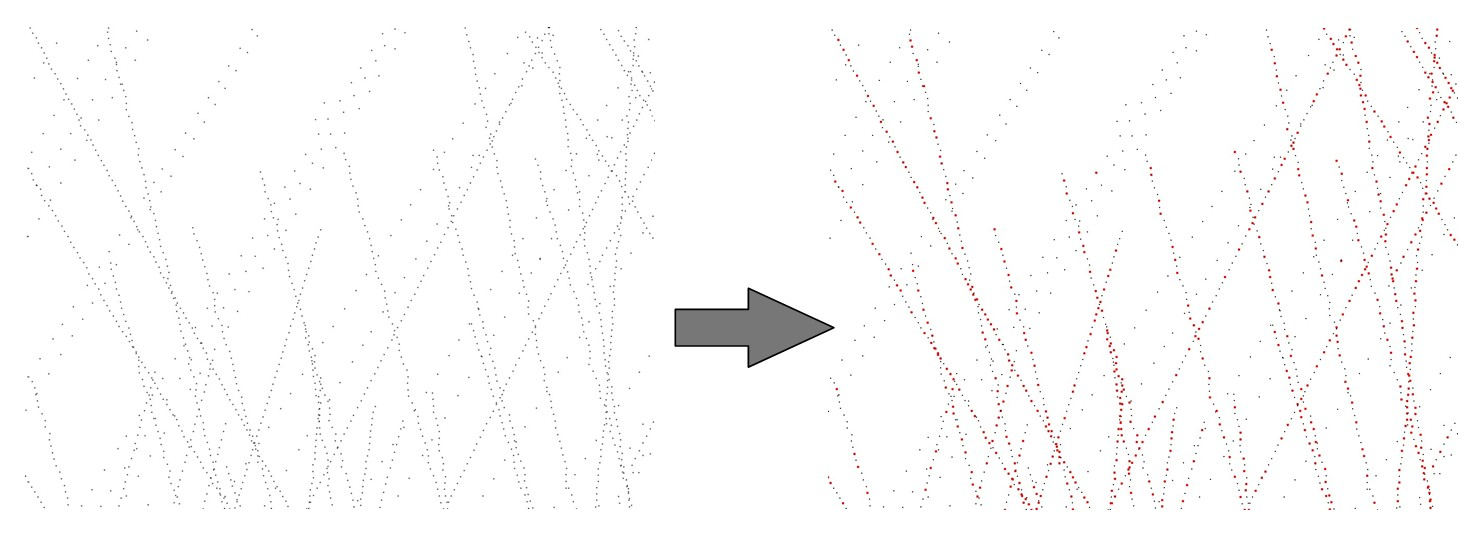
\includegraphics[width=1.0\textwidth]{Point_set_processing_3/merge_simplification} % omit .eps suffix
    \end{ccTexOnly}
    \begin{ccHtmlOnly}
        <img width="100%" border=0 src="../Point_set_processing_3/merge_simplification.jpg"><P>
    \end{ccHtmlOnly}
    % Title
    \begin{figure}[h]
        \caption{Point set implification through grid-based clustering.
                 Left: input point set.
                 Right: removed points are depicted in red.}
    \end{figure}
\end{center}



